% !TeX root = ../main.tex

\section{Automazione del Processo di Sviluppo}

\begin{frame}{Pratiche DevOps}
    \begin{columns}[onlytextwidth]
        \begin{column}{0.45\textwidth}
    
            \textbf{Continuous Integration}
            \begin{itemize}
                \item \textbf{Stages}:
                \begin{itemize}
                    \item Build
                    \item Test
                    \item Package
                \end{itemize}
            \end{itemize}

            \vspace{4mm}

            \textbf{Continuous Delivery}:
            \begin{itemize}
                \item \textbf{Stages}:
                \begin{itemize}
                    \item Release alpha
                    \item Release beta
                    \item Release prod
                \end{itemize}
            \end{itemize}
            
        \end{column}
        \begin{column}{0.45\textwidth}

            \textbf{Obiettivo}:
            \begin{itemize}
                \item Dalla modifica al rilascio nel minor tempo possibile
                \item Verifica delle modifiche
                \item Riuso (Template)
                \item Estensione (Pipeline-as-Code)
            \end{itemize}
        
        \end{column}
    \end{columns}

    \vspace{2mm}

    \begin{figure}[H]
        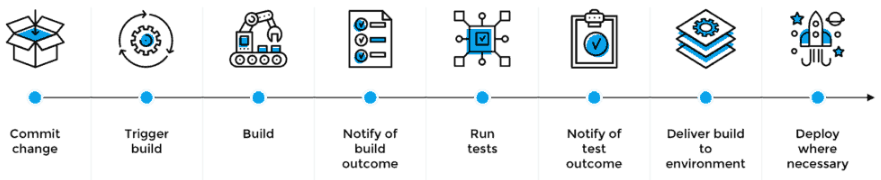
\includegraphics[width=0.9\textwidth]{img/cicd.png}
    \end{figure}
    
\end{frame}

\begin{frame}{Sistema Complessivo}

    \begin{figure}[H]
        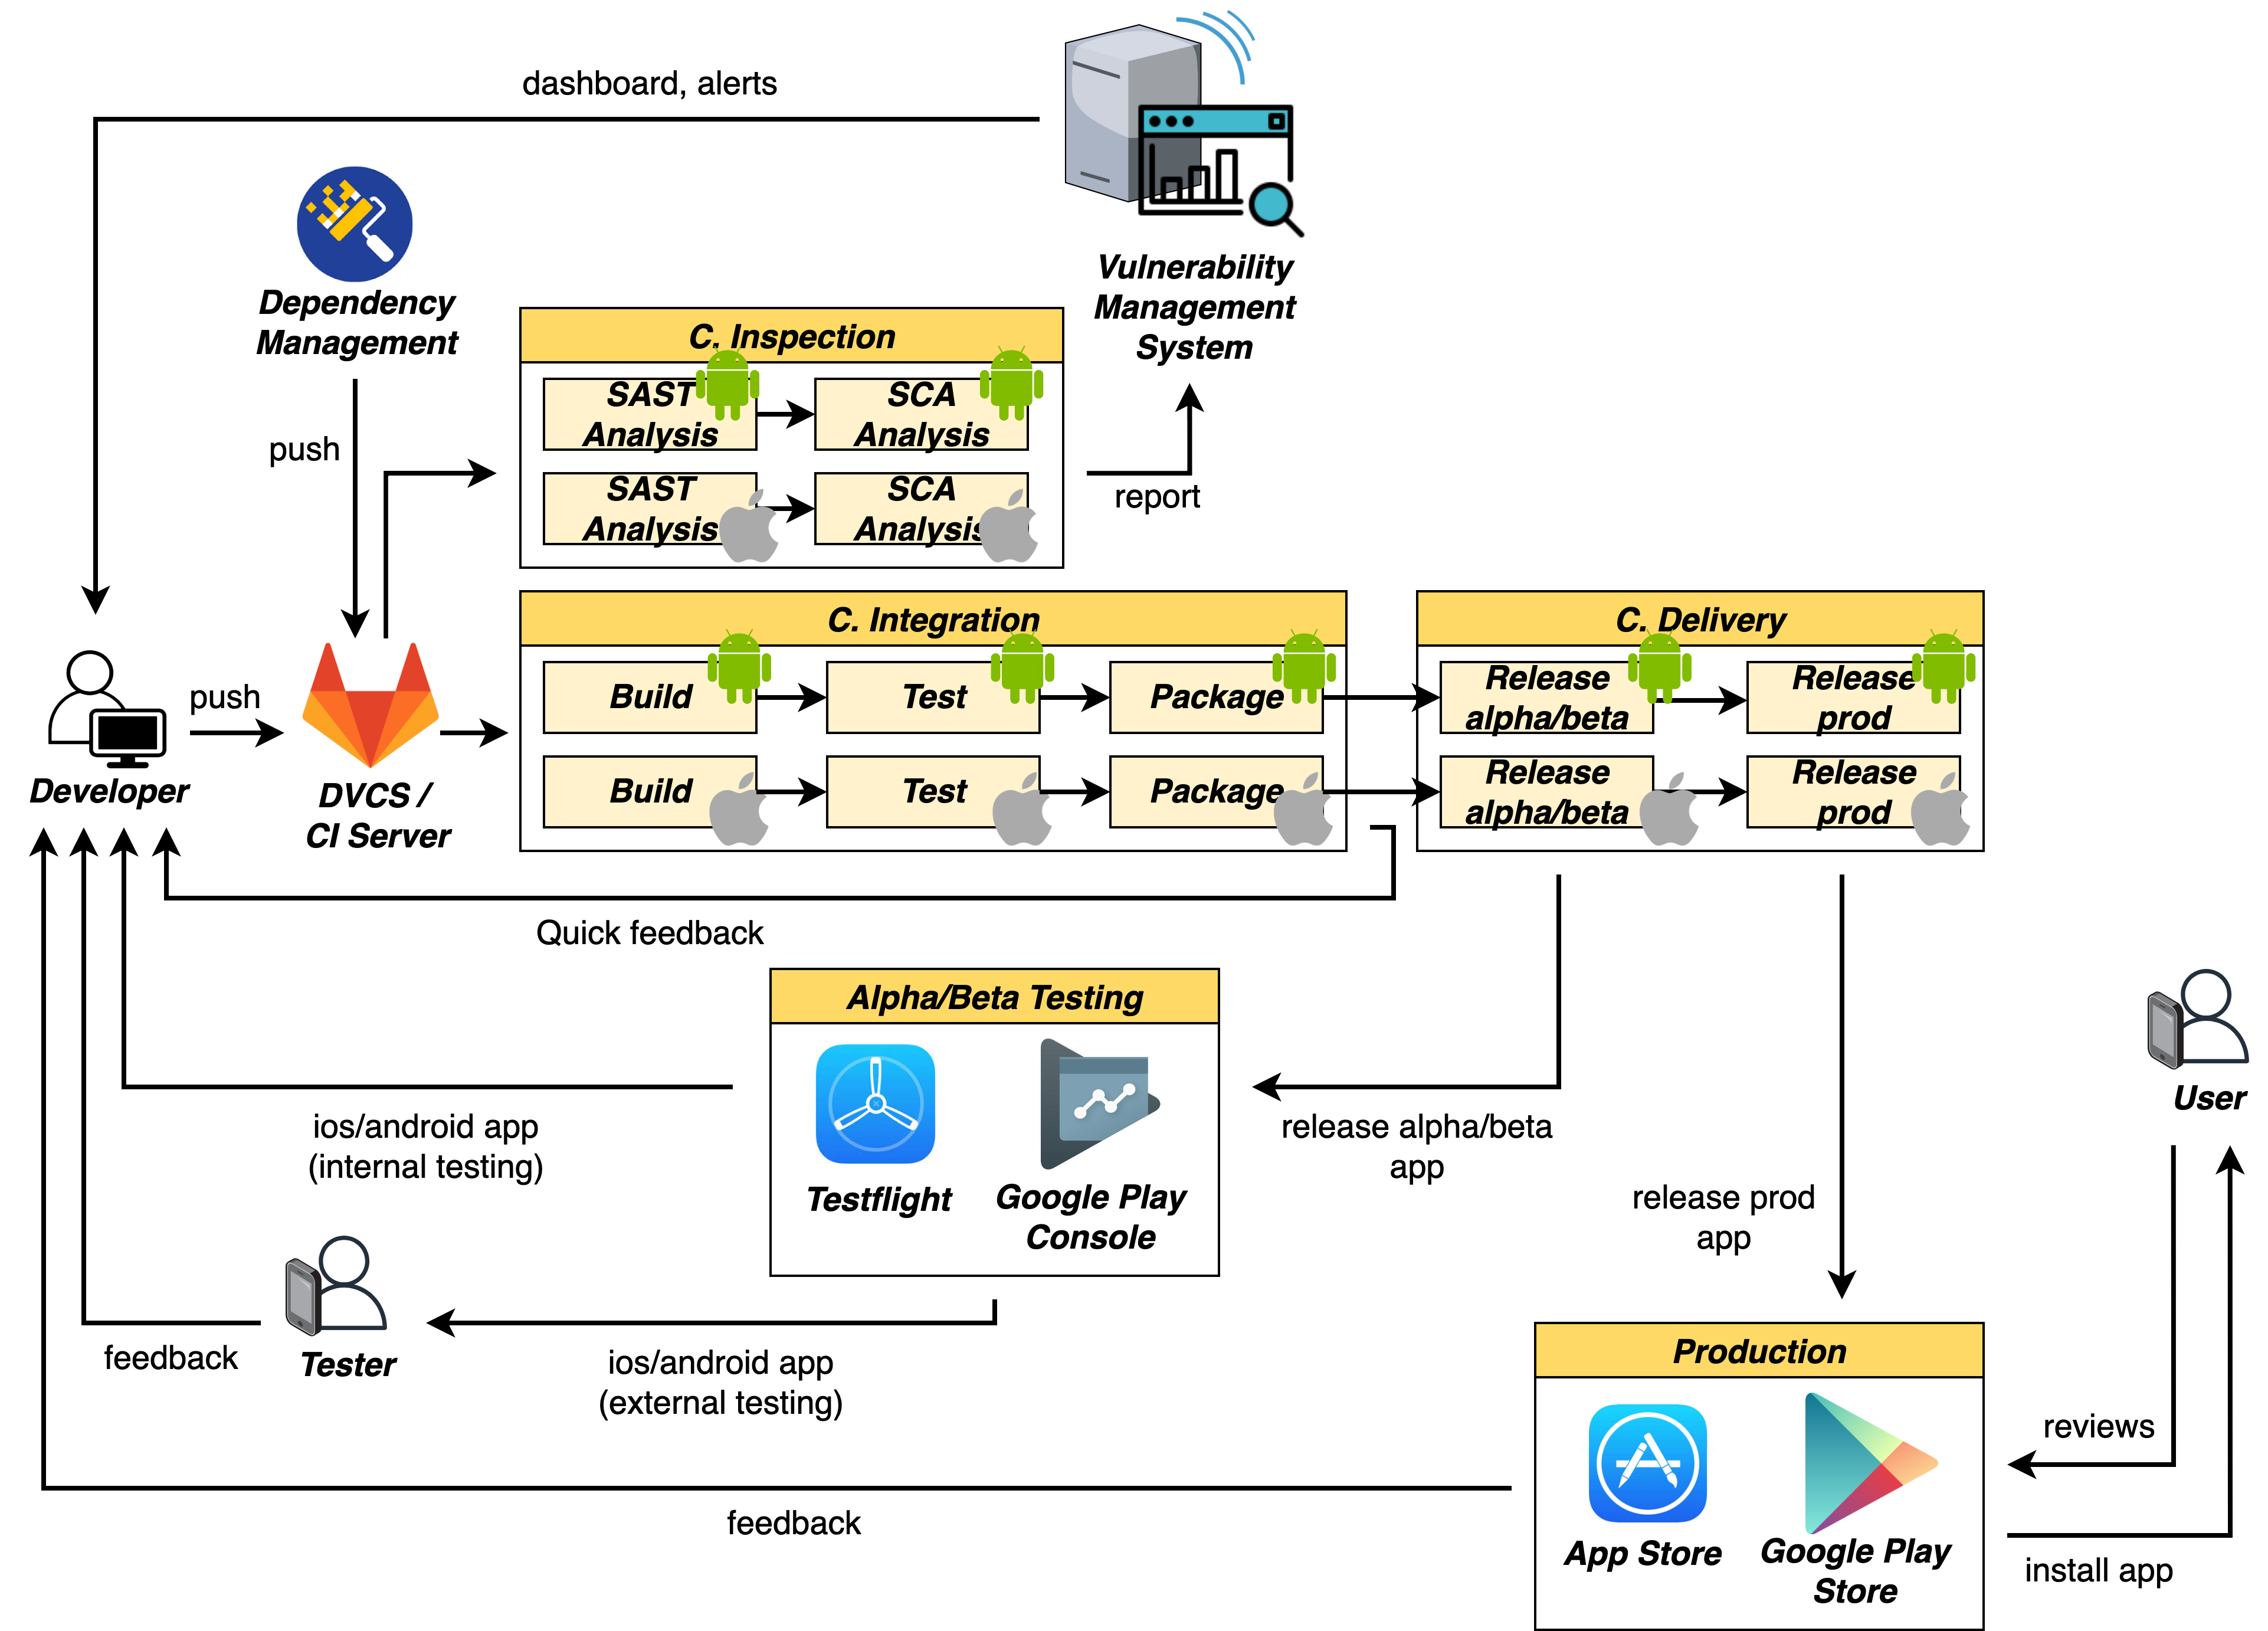
\includegraphics[width=0.85\textwidth]{img/full-cicd.png}
    \end{figure}

\end{frame}